\section{What is Planning?}
\label{sect:planning_intro}
We distinguish planning from prediction for software quality as follows: 
Quality prediction points to the likelihood of defects. Predictors take the form:
\begin{equation*}
  out = f(in)  
\end{equation*}
where {\em in} contains many independent features (such as OO metrics) and {\em out} contains some measure of
how many defects are present. For software analytics, the function $f$ is learned via mining static code attributes.

% \begin{figure}[!t]
%     \centering
%     \includegraphics[width=\linewidth]{images/example.png}
%     \caption{A proposed planning framework.}
%     \label{fig:flowchart}
% \end{figure}

\begin{figure}
\centering
\captionsetup[subfigure]{width=\linewidth}
\subfloat[subfig:plans][Recommendations from some planner. 
The terms highlighted in the first row come from Figure~\ref{fig:static_metrics}.
In the second row, 
 a `$+$' represents an \textit{increase}; a `$-$'  represents an \textit{decrease};  and a `$\cdot$' represents \textit{no-change}.]{
\resizebox{0.8\linewidth}{!}{
\begin{tabular}{ccccccccc}
\hline
\rowcolor{Gray} DIT & NOC & CBO & RFC & FOUT & WMC & NOM & LOC & LCOM \\
$\cdot$ & $\cdot$    & $\cdot$    & $+$   & $\cdot$     & $+$   & $+$   & $+$   & $+$    \\\hline
\end{tabular}}
\label{subfig:plans}
}\\

\vspace{5mm}
\subfloat[][A sample of possible actions developers can take.
 Here a `$+$' represents an \textit{increase}, a `$-$' represents a \textit{decrease}, and an empty cell represents \textit{no-change}.
Taken from~\cite{stroggylos2007, du2006study, kataoka2002, bryton2009,elish2011,elish2012}. The action highlighted in \colorbox{lightgray}{gray} shows an  action matching XTREE's   recommendation
from Figure~\ref{fig:motivating_example}.A.]{
\resizebox{\linewidth}{!}{
\begin{tabular}{lccccccccc}
\hline
\rowcolor{Gray}Action                                      & DIT & NOC & CBO & RFC & FOUT & WMC & NOM & LOC & LCOM \\ 
Extract Class                               &     &     & $+$   & $-$   & $+$    & $-$   & $-$   & $-$   & $-$    \\
\rowcolor{lightgray} Extract Method                              &     &     &     & $+$   &      & $+$   & $+$   & $+$   & $+$    \\
Hide Method                                 &     &     &     &     &      &     &     &     &      \\
Inline Method                               &     &     &     & $-$   &      & $-$   & $-$   & $-$   & $-$    \\
Inline Temp                                 &     &     &     &     &      &     &     & $-$   &      \\
Remove Setting Method                       &     &     &     & $-$   &      & $-$   & $-$   & $-$   & $-$    \\
Replace Assignment                          &     &     &     &     &      &     &     & $-$   &      \\
Replace Magic Number                        &     &     &     &     &      &     &     & $+$   &      \\
Consolidate Conditional                     &     &     &     & $+$   &      & $+$   & $+$   & $-$   & $+$    \\
Reverse Conditional                         &     &     &     &     &      &     &     &     &      \\
Encapsulate Field                           &     &     &     &     &      & $+$   & $+$   & $+$   & $+$    \\
Inline Class                                &     &     & $-$   & $+$   & $-$    & $+$   & $+$   & $+$   & $+$    \\ \hline
\end{tabular}}
\label{subfig:actions}
}\\

\vspace{5mm}
\subfloat[Before `extract method'][Before `extract method']{
\fbox{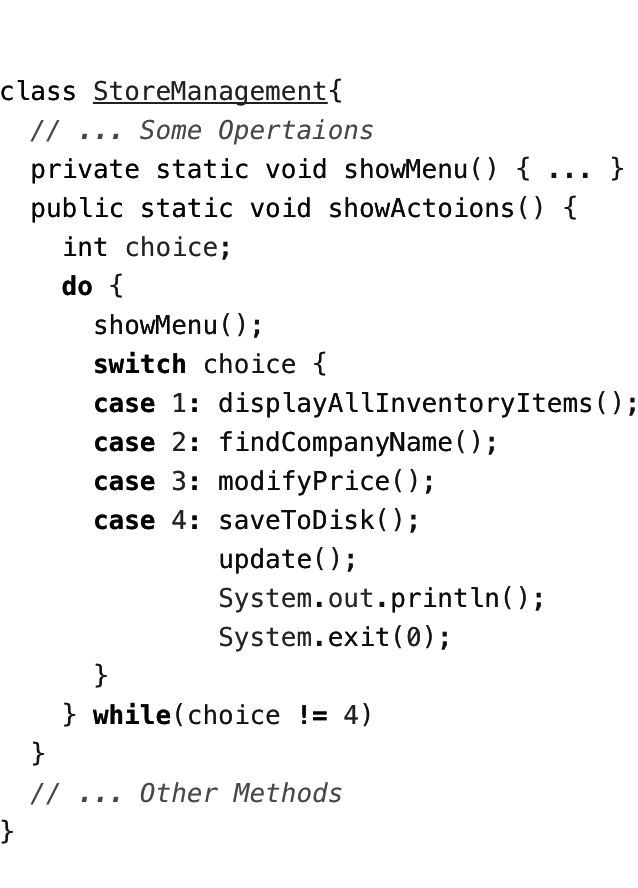
\includegraphics[width=0.45\linewidth]{1.png}}
\label{subfig:before}
}
\subfloat[After `extract method'][After `extract method']{
\fbox{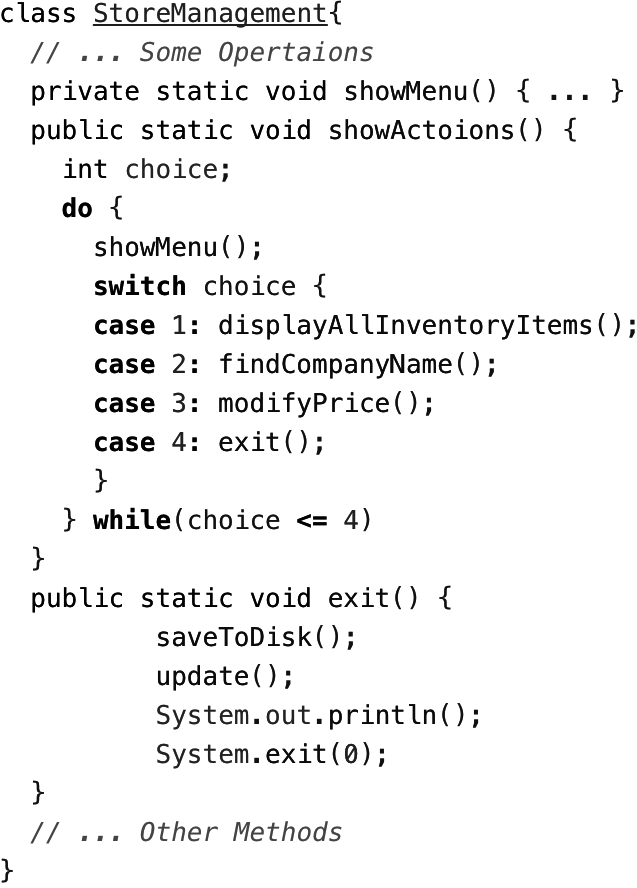
\includegraphics[width=0.45\linewidth]{2.png}}
\label{subfig:after}
}

\caption{An example of how developers might use XTREE to reduce software defects.}
\label{fig:motivating_example}
\end{figure}

On the other hand, quality planning seeks  precautionary measures to significantly reduce the likelihood of future defects.

For a formal definition of plans, consider a defective test example $Z$, a planner
proposes a plan ``$\Delta$'' to adjust attribute $Z_j$ as follows:

{\small\[
\forall \delta_j \in \Delta : Z_j = 
\begin{cases}
   Z_j \pm \delta_j& \text{if $Z_j$ is numeric}\\
  \delta_j       & \text{otherwise}
\end{cases}
\]}

The above plans are described in terms of a range of numeric values. In this case, they represent an increase (or decrease) in some of the static code metrics of \tab{static_metrics}. However, these numeric ranges in and of themselves may not very informative. It would be beneficial to offer a more detailed report on how to go about implementing these plans. For example, to (say) simplify a large bug-prone method, it may be useful to suggest to a developer to reduce its size (e.g., by splitting it across two simpler functions).


In order to operationalize such plans, developers need some guidance on what to change in order to achieve the desired effect. 
There are two places to look
for that guidance:
\be
\item In other projects;
\item In the current project.
\ee
As to  the first approach
({\em using other projects}), 
 several recent papers have discussed how code changes adjust
static code metrics~\citep{stroggylos2007, du2006study, kataoka2002, bryton2009, elish2011, elish2012}.
For example,
\fig{motivating_example}(b) shows a summary of
that research. 
We could apply those results
as follows:\bi
\item
Suppose a planner has recommended the changes shown in \fig{motivating_example}(a). 
\item
Then, we use \ref{fig:motivating_example}\protect\subref{subfig:actions} to look-up possible actions developers may take.
Here, we see that performing an ``extract method'' operation may help alleviate certain defects (this is highlighted in {\colorbox{lightgray}{gray}}).
\item
In \ref{fig:motivating_example}\protect\subref{subfig:before} we show a simple example of a class where the above operation may be performed. 
\item
In \ref{fig:motivating_example}\protect\subref{subfig:after}, we demonstrate how a developer may perform the ``extract method''. 
\ei
% several
% recent papers propose lists
% of programmer actions that result
% in particular kinds of changes to
% our metrics~\citep{stroggylos2007, du2006study, kataoka2002, bryton2009,krishna2017less}.
% For example, Stroggylos \& Spinellis~\citep{stroggylos2007} studied the impact of CK-metrics to assert if performing reorganization was useful in reducing bugs and improving software quality.
% They reported a strong correlation between these metrics and software quality. Du Bois~\citep{du2006study} conducted a study that explored coupling and cohesion metrics and reported similar findings. Elish \& Alshayeb~\citep{elish2011, elish2012} conducted a systematic study to categorize code reorganization procedures in terms of their measurable effect on software quality attributes. Their studies showed how each reorganization action would impact several of the CK-metrics. 
% Although these and other similar studied were enlightening in that they demonstrated the strong correlation between static code metrics and the reorganization, a major shortcoming of these approaches is that they left much of the decision making to the developers. Numerous recent studies challenge this approach. Consider the findings of Devanbu et al.~\citep{devanbu2016belief}, who, after examining responses from 564 Microsoft developers around the world, showed that the some of the most ardent beliefs held by developers must now be carefully re-examined in the face of new empirical evidence. This work is response to these and other similar criticisms. The remainder of this section provide an example of how our proposed method addresses this issue.
% Our framework attempts to automate the process of decision making by reflecting on past releases of the software projects. To do this, we adopt two strategies, the first of which was 
While using other projects may be useful,
that approach has a problem. Specifically: 
what happens
 if the proposed change has not been studied before in the literature?
 For this reason,
 we prefer to use the second approach
 (i.e. {\em use the current project}).
 In that approach, we look through the developer's own history to find old examples where they have made the kinds of changes recommended by the plan. 
Other researchers also adopt this approach (see
\citep{nayrolles2018clever} at MSR 2018). In the following:
 \bi
 \item
Using frequent itemset  mining, we
   summarize prior  changes in the current
 project (for details on this kind of learning, see 
  \fig{xtree}.C).
 \item
Next, when we learn plans, we reject any
that are not known prior changes.
\ei
 In this way, we can ensure that if a developer asks ``how do I implement this plan?'',
 we can reply with a relevant
 example of prior changes to the current project.


\subsection{Planning in Software Engineering}
\label{sect:planners}

We say that \fig{motivating_example} is an example of {\em code-based planning} where the goal is to change a code base in order to improve that code in some way. The rest of this section first discusses other kinds of planning before discussing \textit{code based planning} in greater detail.

Planning is extensively explored in artificial intelligence research. There, it usually refers to generating a sequence of actions that enables an \textit{agent} to achieve a specific \textit{goal}~\citep{norvig}. This can be achieved by classical search-based problem solving approaches or logical planning agents. Such planning tasks now play a significant role in a variety of demanding applications, ranging from controlling space vehicles and robots to playing the game of bridge~\citep{ghallab04}. Some of the most common planning paradigms include: (a) classical planning~\citep{wooldridge95}; (b) probabilistic planning~\citep{Bel, altman99, guo2009}; and (c) preference-based planning~\citep{son06, baier09}. Existence of a model precludes the use of each of these planning approaches. This is a limitation of all these planning approaches since not every domain has a reliable model. 

We know of at least two two kinds of planning research in software engineering. Each kind is distinguishable by {\em what} is being changed.
\bi
\item
In {\em test-based planning}, some optimization is applied to reduce the number of tests required to achieve to a certain goal or the time taken before tests yield interesting results~\citep{tallam2006concept, yoo2012regression, blue2013interaction}.
\item
In {\em process-based planning} some search-based optimizer is applied to a software process model to infer high-level business plans about software projects. Examples of that kind of work include our own prior studies sarching over  COCOMO models~\cite{me07f,Menzies:2009:ADS} or Ruhe et al.'s work on next release planning in requirements engineering~\citep{ruhe2003quantitative, ruhe2010product}. 
\ei
In software engineering, the planning problem translates to proposing changes to software artifacts. These are usually a hybrid task combining probabilistic planning and preference-based planning using search-based software engineering techniques~\citep{Harman2009, Harman2011}. These search-based techniques are evolutionary algorithms that propose actions guided by a fitness function derived from a well established domain model. Examples of algorithms used here include GALE, NSGA-II, NSGA-III, SPEA2, IBEA, MOEA/D, etc.~\citep{krall2015gale, deb00a, zit02, zit04, deb14, Cui2005a, zhang07:TEC}. 
As with traditional planning, these planning tools all require access to some trustworthy models that can be used to explore some highly novel examples. In some software engineering domains there is ready access to such models which can offer assessment of newly generated plans. Examples of such domains within software engineering include automated program repair~\citep{Weimer2009, Goues12, LeGoues2015}, software product line management~\citep{sayyad13, metzger14, henard15}, automated test generation~\citep{andrews07, andrews10}, etc. 

However, not all domains come with ready-to-use models. For example, consider all the intricate issues that may lead to defects in a product. A model that includes {\em all} those potential issues would be very large and complex. Further, the empirical data required to validate any/all parts of that model can be hard to find. Worse yet, our experience has been that accessing and/or commissioning a model can be a labor-intensive process. For example, in previous work~\citep{me07f} we used models developed by Boehm's group at the University of Southern California.Those models took as inputs project descriptors to output predictions of development effort, project risk, and defects.
Some of those models took decades to develop and mature (from 1981~\citep{boehm81} to 2000~\citep{boehm00b}). Lastly, even when there is an existing model, they can require constant maintenance lest they become out-dated. Elsewhere, we have described our extensions to the USC models to enable reasoning about agile software developments. It took many months to implement and certify those extensions~\citep{me09i, me09j}. The problem of model maintenance is another motivation to look for alternate methods that can be quickly and automatically updated whenever new data becomes available.

In summary, for domains with readily accessible models, we recommend the kinds of tools that are widely used in the search-based software engineering community such as GALE, NSGA-II, NSGA-III, SPEA2, IBEA, particle swarm optimization, MOEA/D, etc. In other cases where this is not an option, we propose the use of data mining approaches to create a quasi-model of the domain and make use of observable states from this data to generate an estimation of the model. Examples of such a data mining approaches are described below. These include five methods described in the rest of this paper: 
\bi
\item Our approaches: XTREE, BELLTREE, and 
\item Three other approaches: Alves et al.~\citep{alves}, Shatnawi~\citep{shatnawi}, and Oliveira et al.~\citep{oliveira} 
\ei

\subsection{Code based Planning}
Looking through the SE literature, we can see that researchers have proposed three methods that rely on \textit{outlier statistics} to identify suitable changes to source code metrics. The general principle underlying each of these methods is that any metric has an \textit{unusually} large (or small) value needs to be change so as not to have such large (or small) values. The key distinction between the methods is how they determine what the threshold for this unusually large  (or small) value ought to be. These methods, proposed by Alves et al.~\citep{alves}, Shatnawi~\citep{shatnawi}, and Oliveira et al.~\citep{oliveira}, are described in detail below.


\subsubsection{Alves}
Alves et al.~\citep{alves} proposed an unsupervised approach
that uses the underlying statistical 
distribution and scale of the OO metrics. It works by first weighting each metric value according to the source lines of 
code (SLOC) of the class it belongs to. All the weighted metrics are then normalized by the sum of all weights for the system. The normalized metric values are ordered in an ascending fashion (this is
equivalent a density function, where the x-axis represents 
the weight ratio (0-100\%), and the y-axis the metric scale).

Alves et al. then select a percentage value (they suggest 70\%) which 
represents the ``normal'' values for metrics. The metric threshold, then, 
is the metric value for which 70\% of the classes fall below. The 
intuition is that the worst code has outliers beyond 70\% of the normal 
code measurements i.e., they state that the risk of there existing a defect 
is moderate to high when the threshold value of 70\% is exceeded.

Here, we explore the correlation between the code metrics 
and the defect counts with a univariate logistic regression and reject 
code metrics that are poor predictors of defects (i.e.  those with $p > 
0.05$). For the remaining metrics, we obtain the threshold ranges which are denoted by $[0, 70\%)$ ranges for each metric. The plans would then involve reducing these metric range to lie within the thresholds discovered above.

\subsubsection{Shatnawi}

Shatnawi~\citep{shatnawi} offers a different alternative Alves et al by using VARL (Value of Acceptable Risk Level). This method was initially proposed by Bender~\citep{bender99} for his epidemiology studies. This approach uses two constants ($p_0$ and $p_1$) to compute the thresholds, which Shatnawi recommends to be set to $p_0=p_1=0.05$. Then using a univariate binary logistic regression three coefficients are learned:
$\alpha$ the intercept constant;
$\beta$ the coefficient for maximizing log-likelihood;
and $p_0$ to 
measure how well this model predicts for defects. (Note: the univariate 
logistic regression was conducted comparing metrics to defect counts. Any 
code metric with $p>0.05$ is ignored as being a poor defect predictor.)

Thresholds are learned from the surviving metrics using
the risk equation proposed by Bender:
$$ \mathit{Defective\ if}\ \mathit{Metric} > \mathit{VARL}$$
$$
	\mathit{VARL} = p^{-1}(p_0) = \frac{1}{\beta }\left( {\log \left( 
		{\frac{{{p_1}}}{{1 - {p_1}}}} \right) - \alpha } \right)
$$

In a similar fashion to Alves et al., we deduce the threshold ranges as $[0, VARL)$ for each selected metric. The plans would again involve reducing these metric range to lie within the thresholds discovered above.

\subsubsection{Oliveira}
Oliveira et al. in their 2014 paper offer yet another alternative to absolute threshold methods discussed above~\citep{oliveira}. Their method is still unsupervised, but they propose complementing the threshold by a second piece of information called the \textit{relative threshold}. This measure denotes the percentage of entities the upper limit should be applied to. These have the following format:
\[p\%\ of\ the\ entities\ must\ have\ M\leq k\]
Here, $M$ is an OO metric, $k$ is the upper limit of the metric value, and $p$ (expressed as \%) is the minimum percentage of entities are required to follow this upper limit. As an example Oliveira et al. state, ``85\% of the methods should have $CC \leq 14$. Essentially, this threshold expresses that high-risk methods may impact the quality of a system when they represent more than 15\% of the whole population''

The procedure attempts derive these values of $(p, k)$ for each metric $M$. They define a function \texttt{ComplianceRate(p, k)} that returns the percentage of system that follows the rule defined by the relative threshold pair $(p, k)$. They then define two penalty functions: (1) \texttt{penalty1(p, k)} that penalizes if the compliance rate is less than a constant $Min\%$, and (2) \texttt{penalty2(k)} to define the distance between $k$ and the median of preset $Tail$-th percentile. (Note: according to Oliveira et al., median of the tail is an idealized upper value for the metric, i.e., a value representing classes that, although present in most systems, have very high values of M). They then compute the total penalty as \texttt{penalty} = \texttt{penalty1(p, k)} + \texttt{penalty2(k)}. Finally, the relative threshold is identified as the pair of values $(p, k)$ that has the lowest total \texttt{penalty}. After obtaining the $(p, k)$ for each OO metric. As in the above two methods, the plan would involve ensuring the for every metric $M$ $p\%$ of the entities have a value that lies between $(0, k]$. 



